\chapter{Pop the Balloons}

The goal of this game is for the player to pop as many balloons as possible in 30 seconds. The player will have a catapult with the help of which the player will pop the balloons.

\begin{figure}[H]
   \centering
   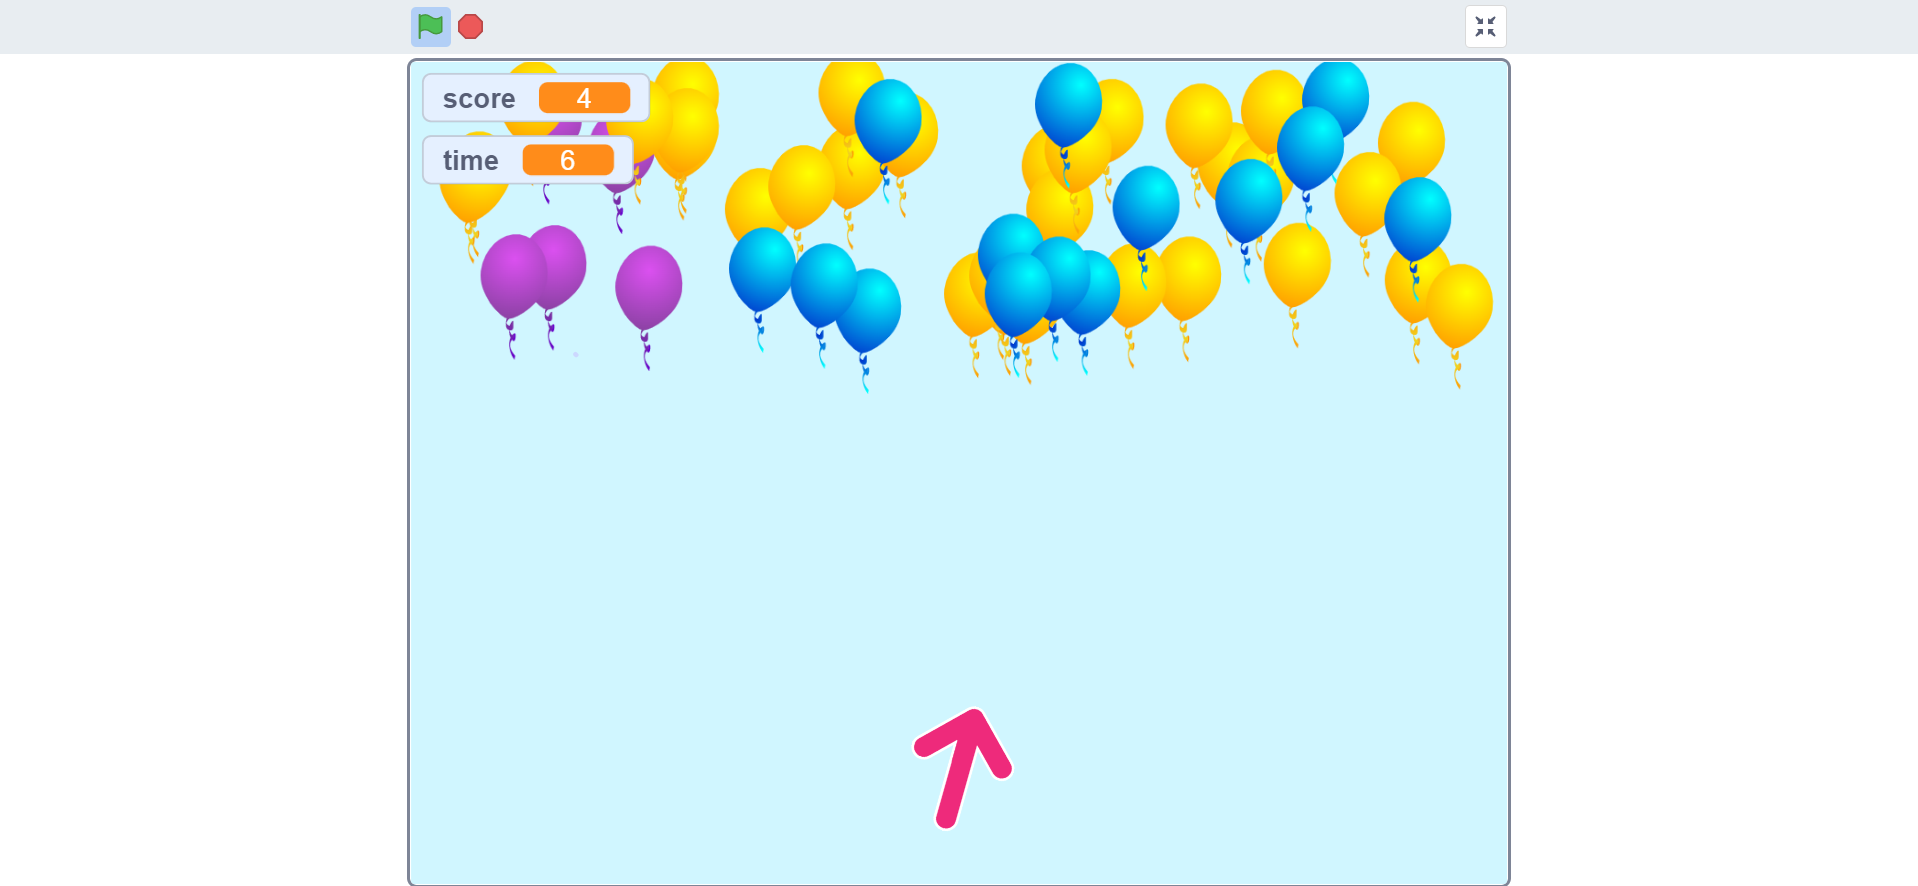
\includegraphics[width=1.0\linewidth,height=0.5\linewidth]{fig090001.png}
   \caption{Pop the balloons}
\label{fig090001}
\end{figure}

\section{Adding Background and Characters}
The first step of the game is to choose a suitable background and characters. The required characters in this game are an arrow representing the catapult, a balloon, and a character announcing the score when the 30 seconds are up.

\begin{figure}[H]
   \centering
   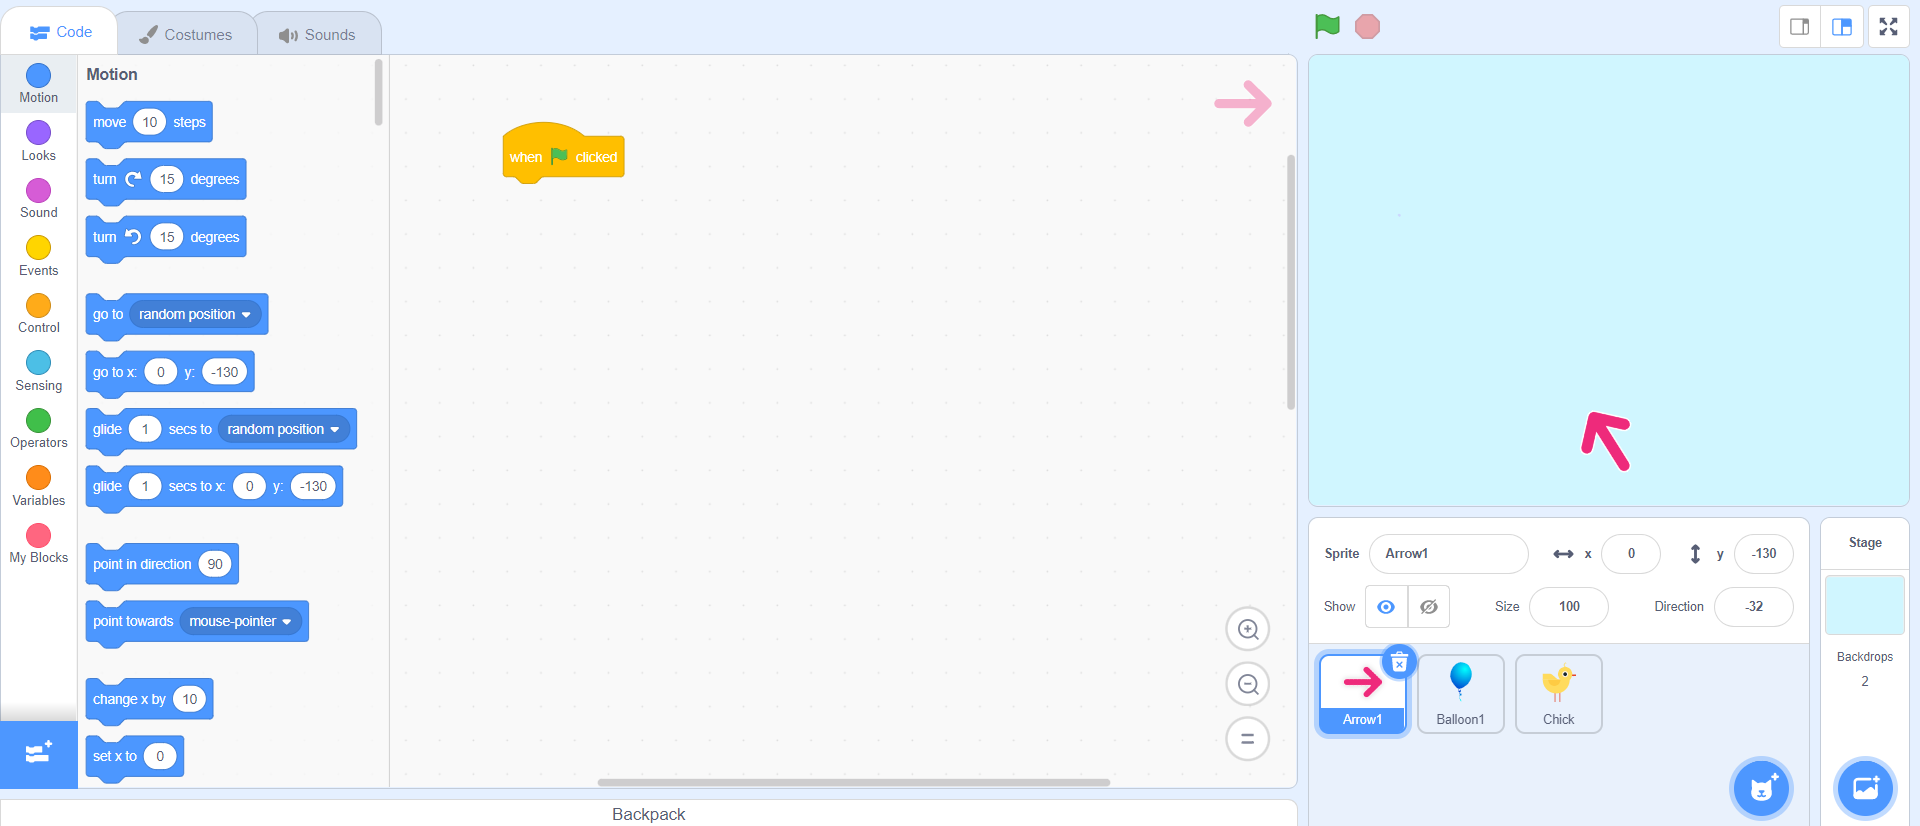
\includegraphics[width=1.0\linewidth,height=0.5\linewidth]{fig090002.png}
   \caption{Adding background and characters}
\label{fig090002}
\end{figure}

\section{Programming the Catapult}
In this game, two variables must be defined - the first will store the time, and the second the score. At the start of the game, the initial value of the time variable should be 30, and the value of the score variable should be 0.

\begin{figure}[H]
   \centering
   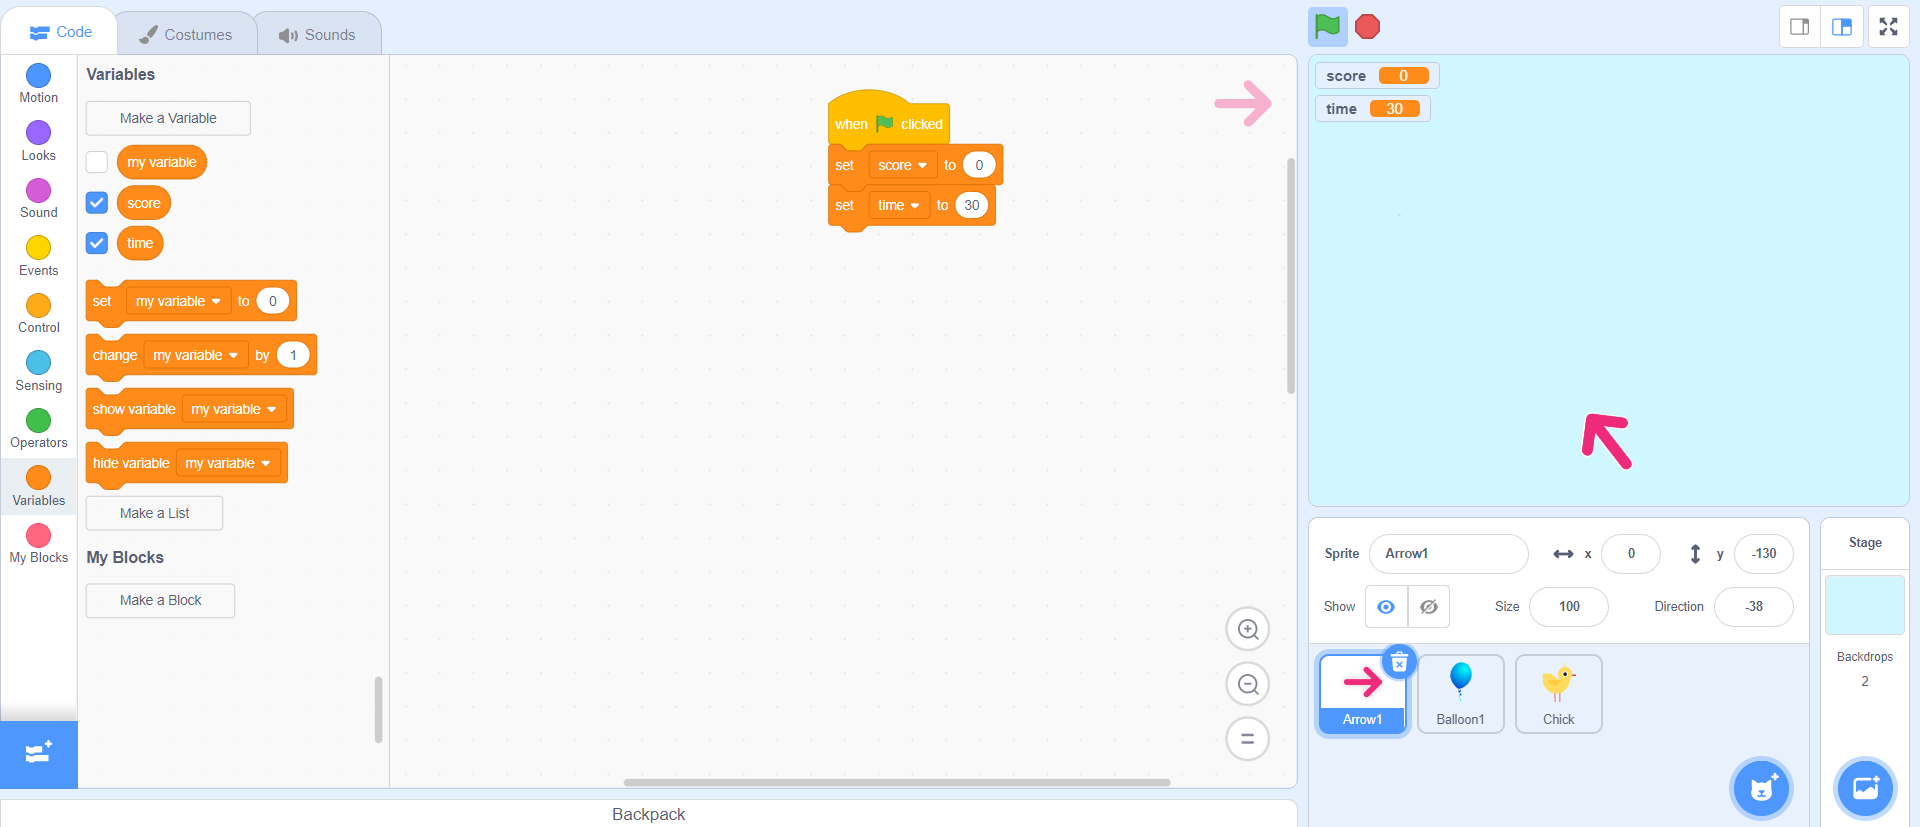
\includegraphics[width=1.0\linewidth,height=0.5\linewidth]{fig090003.png}
   \caption{Initialize variables}
\label{fig090003}
\end{figure}

The game continues until the time variable is equal to 0. It must decrease its value every 1 second.

\begin{figure}[H]
   \centering
   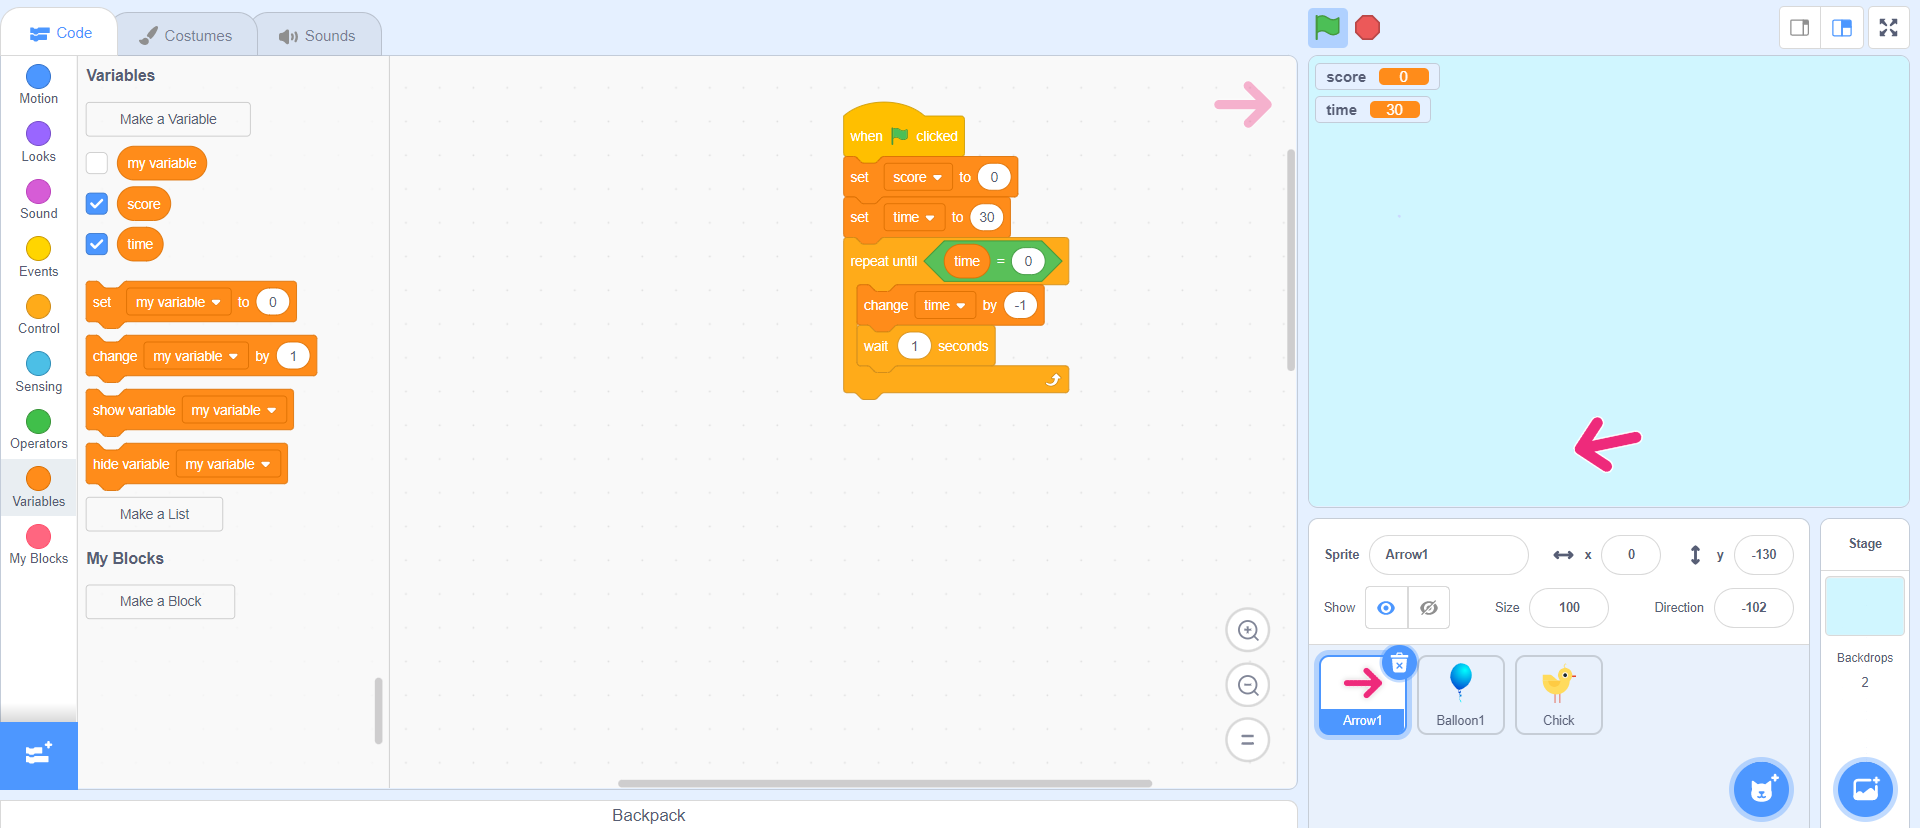
\includegraphics[width=1.0\linewidth,height=0.5\linewidth]{fig090004.png}
   \caption{Change time variable}
\label{fig090004}
\end{figure}

When the time becomes equal to 0, the game is over. Then that character should send a "stop game" message (Fig. \ref{fig090005}. When the game starts, the time variable will be decremented by 1 every second.

\begin{figure}[H]
   \centering
   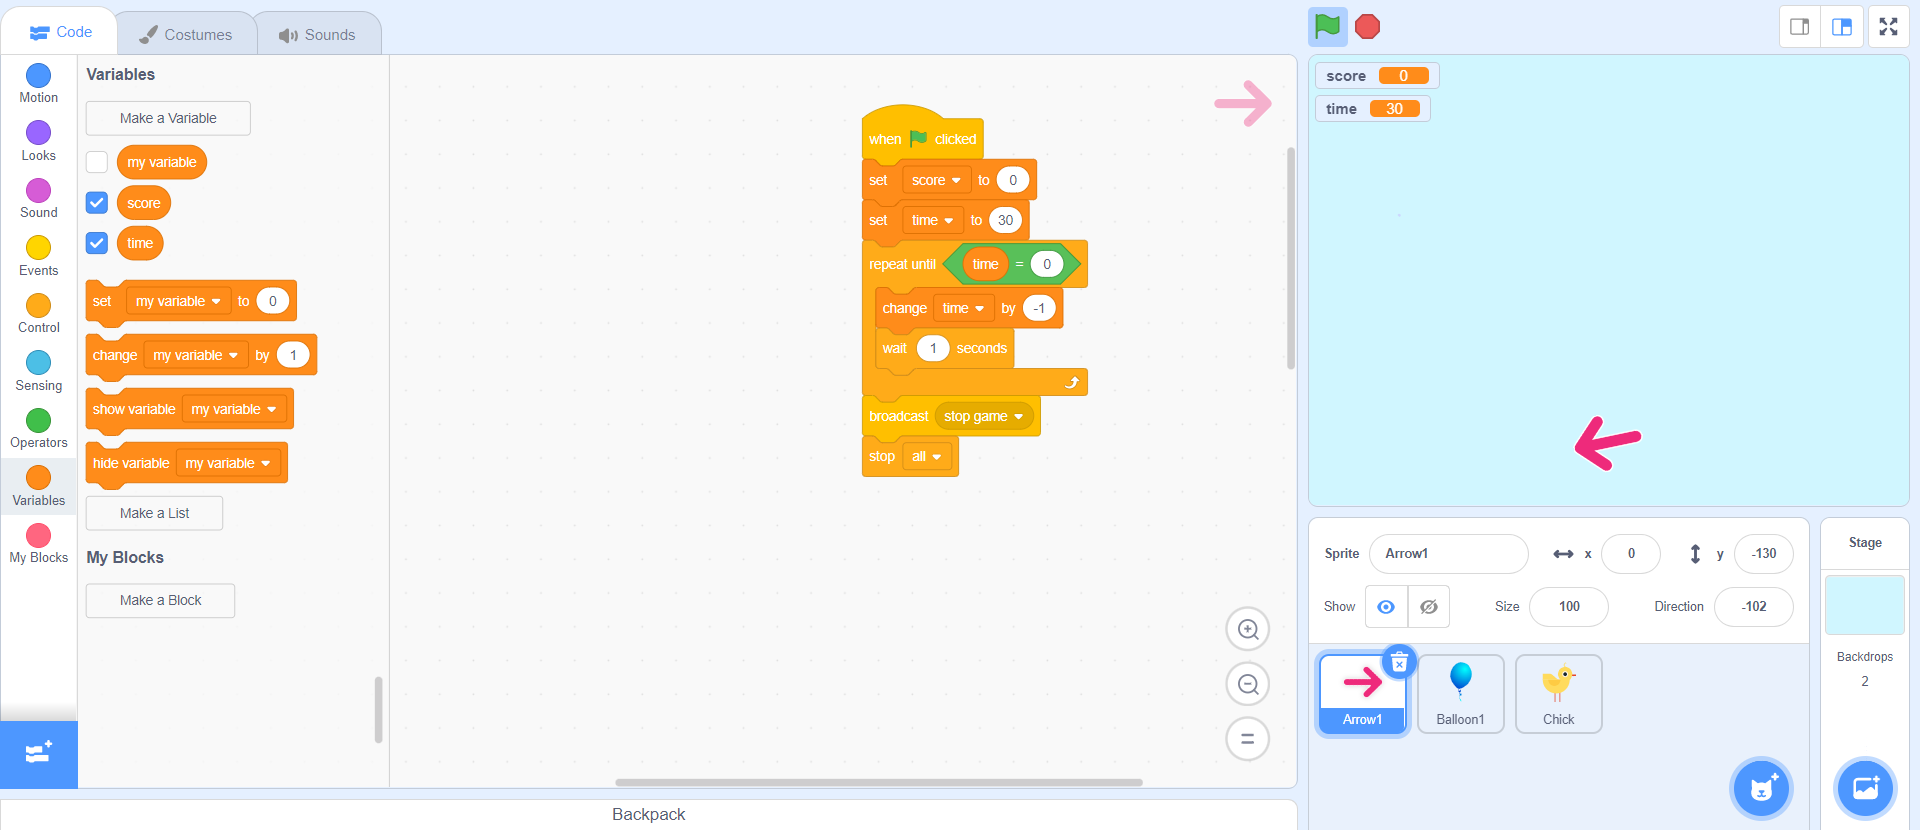
\includegraphics[width=1.0\linewidth,height=0.5\linewidth]{fig090005.png}
   \caption{Send Game End Message}
\label{fig090005}
\end{figure}

During gameplay, the catapult must be positioned at the bottom of the screen and follow the direction of the mouse until the player clicks it. A nested loop must be used, meaning there will be a loop that contains another inside of itself. The outer loop will be infinite. It will end when the game is over. The inner loop will be a loop with a goal, with the goal being until the mouse is clicked. Inside the loop body, the statement should be "point towards mouse-pointer, " meaning "follow the mouse".
 
\begin{figure}[H]
   \centering
   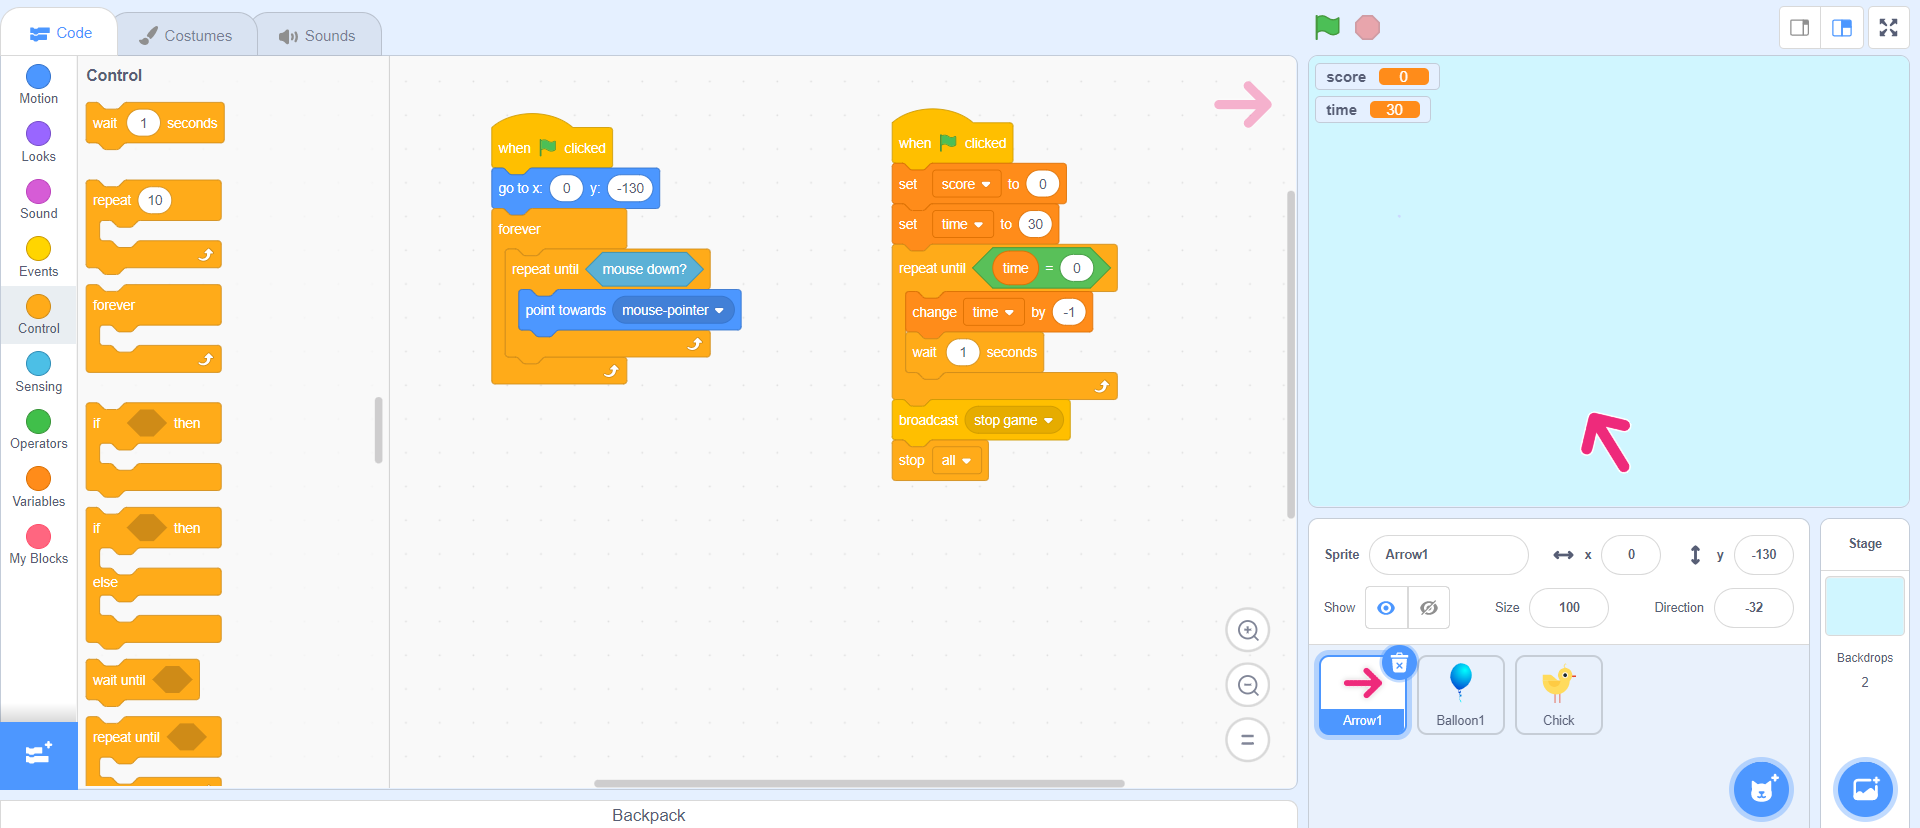
\includegraphics[width=1.0\linewidth,height=0.5\linewidth]{fig090006.png}
   \caption{Mouse Tracking}
\label{fig090006}
\end{figure}

When the game is launched, it is noticed that the catapult follows the direction of the mouse. What remains to be done is when it is clicked to fire, and when it touches any of the edges of the screen, it returns to its original state. Created by instructions, this is done by adding one more inner loop. This time the condition of this loop should be - until the catapult touches some edge of the screen. And in the body of the cycle, the instruction should be placed - it moves by 20 steps. The instructions outside this loop are executed when the character touches the edge. For this, the last instruction is to position the character in a starting position.

\begin{figure}[H]
   \centering
   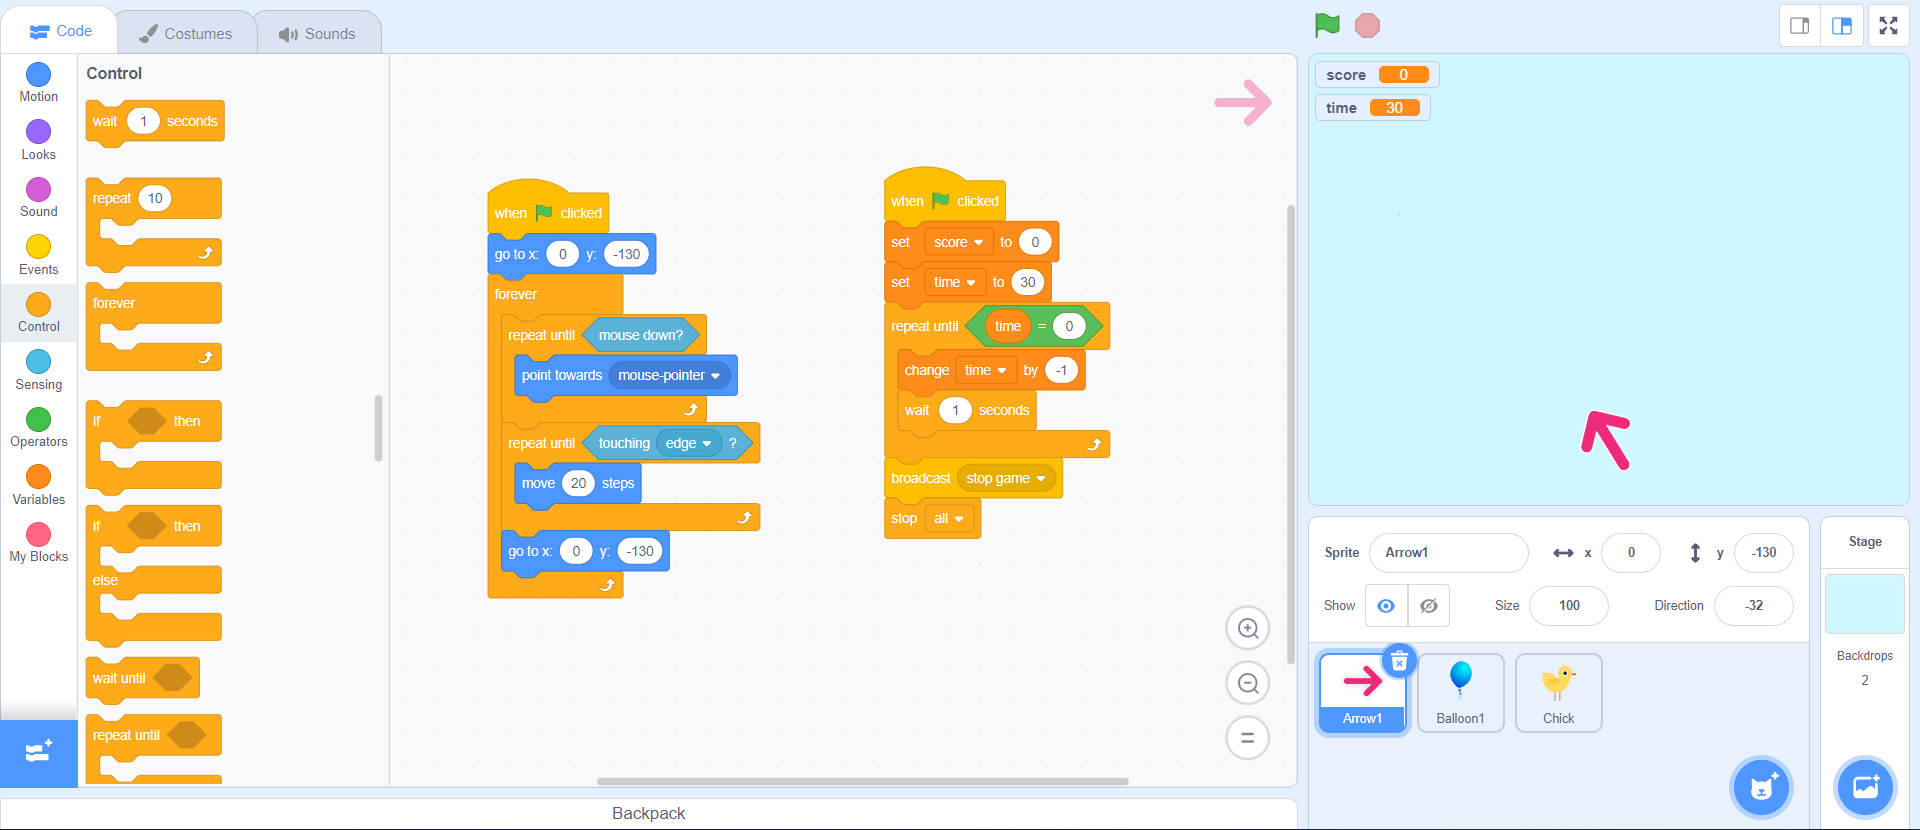
\includegraphics[width=1.0\linewidth,height=0.5\linewidth]{fig090007.png}
   \caption{Final catapult code}
\label{fig090007}
\end{figure}

\section{Programming the Balloon}
In the next step, the instructions for the balloon will also be constructed. Many balloons appear during the game, and the hero is only one. This is done by adding instructions to clone the balloon character. The instructions needed for cloning are in the orange group and are "create a clone of myself" and the instruction "delete this clone".

When the game starts, the original balloon character must hide. His sole purpose is to create clones. Have the bubble create 10 clones of itself, then wait 5 seconds and delete one clone. This algorithm should be repeated 5 times. Here again, the nested loop construct must be used.

\begin{figure}[H]
   \centering
   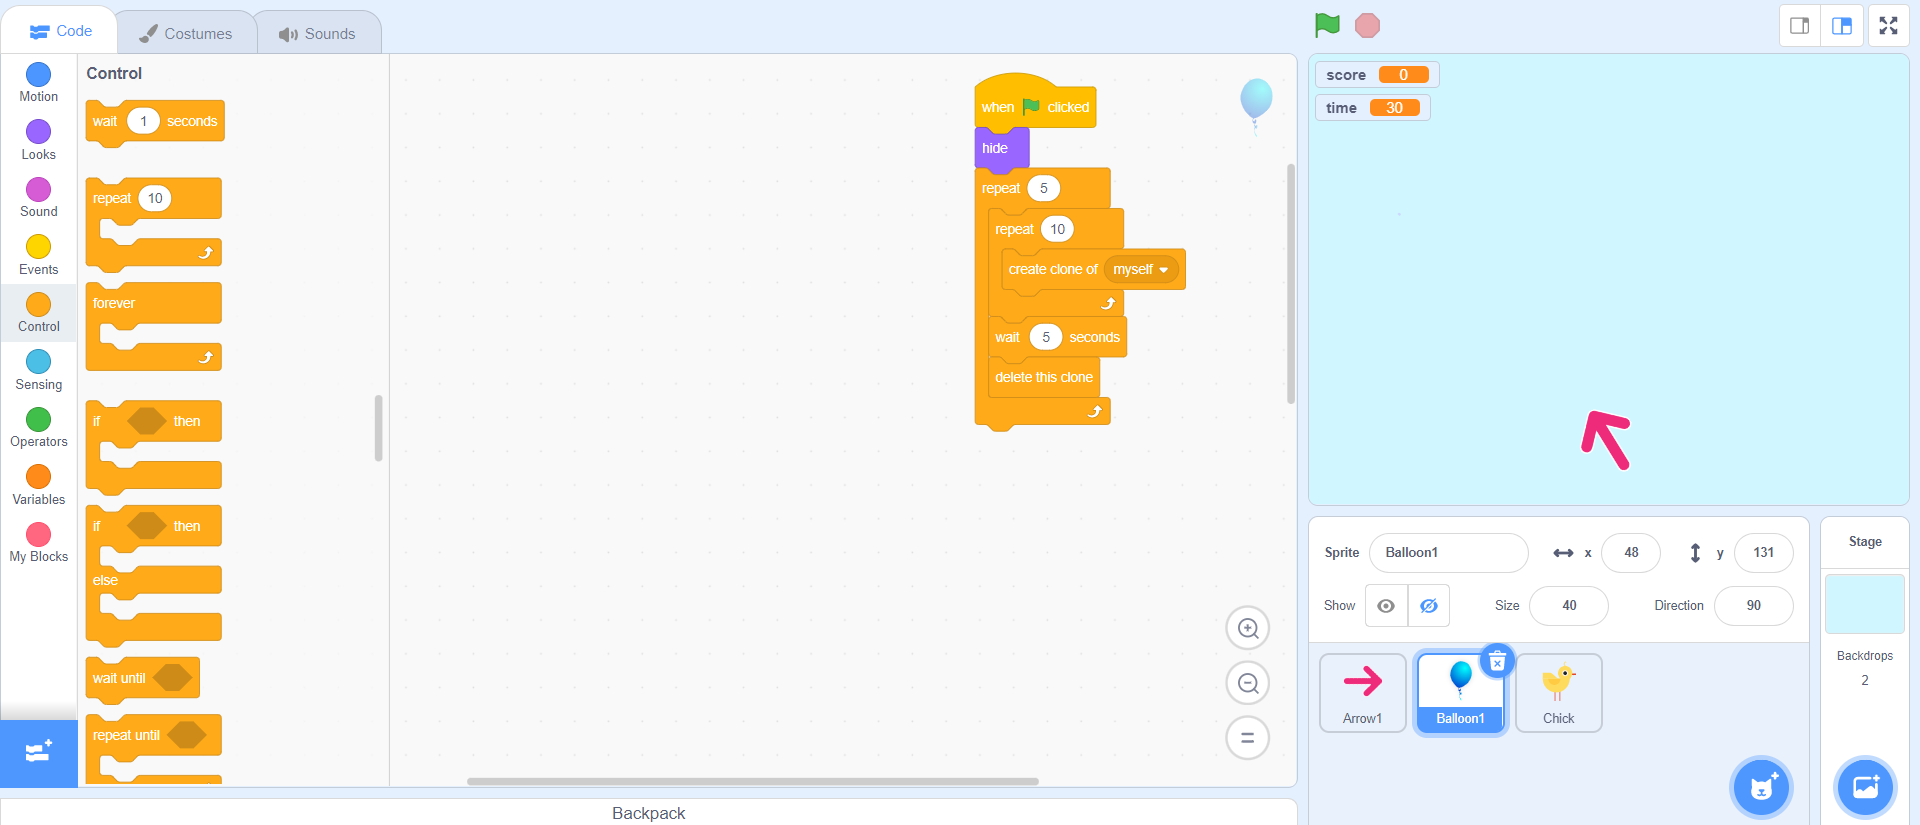
\includegraphics[width=1.0\linewidth,height=0.5\linewidth]{fig090008.png}
   \caption{Clone Creation}
\label{fig090008}
\end{figure}

The balloon clone should also be programmed. From the orange group, the instruction "When I start as a clone" should be used, which means "When I start a clone". The first thing to do is position the clone. To make the game more interesting, let its position be random but at the top of the screen. This means that the number for the x-coordinate should be randomly between -200 and 200 (that's the borders of the screen), and the y-coordinate should be between 50 and 150 (the top of the screen).

Once positioned, the clone should be displayed and resized to be smaller. The two instructions are located in the purple instruction group.

\begin{figure}[H]
   \centering
   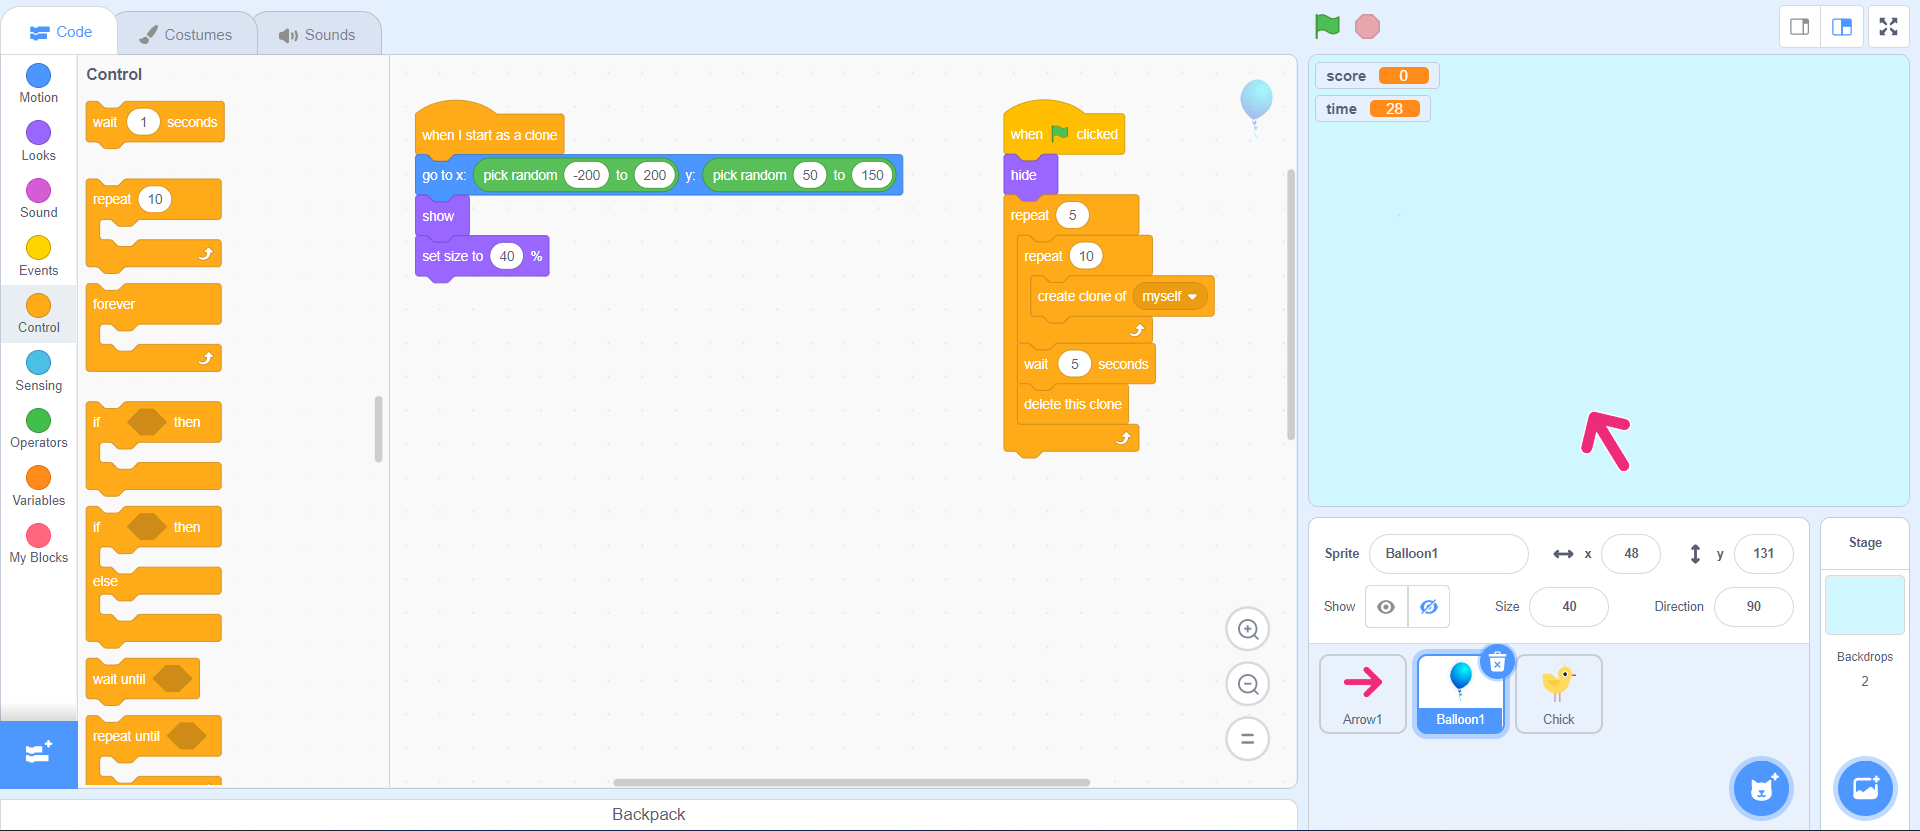
\includegraphics[width=1.0\linewidth,height=0.5\linewidth]{fig090009.png}
   \caption{Clone Positioning}
\label{fig090009}
\end{figure}

Once the bubble appears, it must move one step. In addition to the balloon's movement, two checks must be made. One check is to see if the arrow has touched the clone. If the condition is true, then the value of the result variable should be incremented by 1, and the bubble should be placed at a random position again.

\begin{figure}[H]
   \centering
   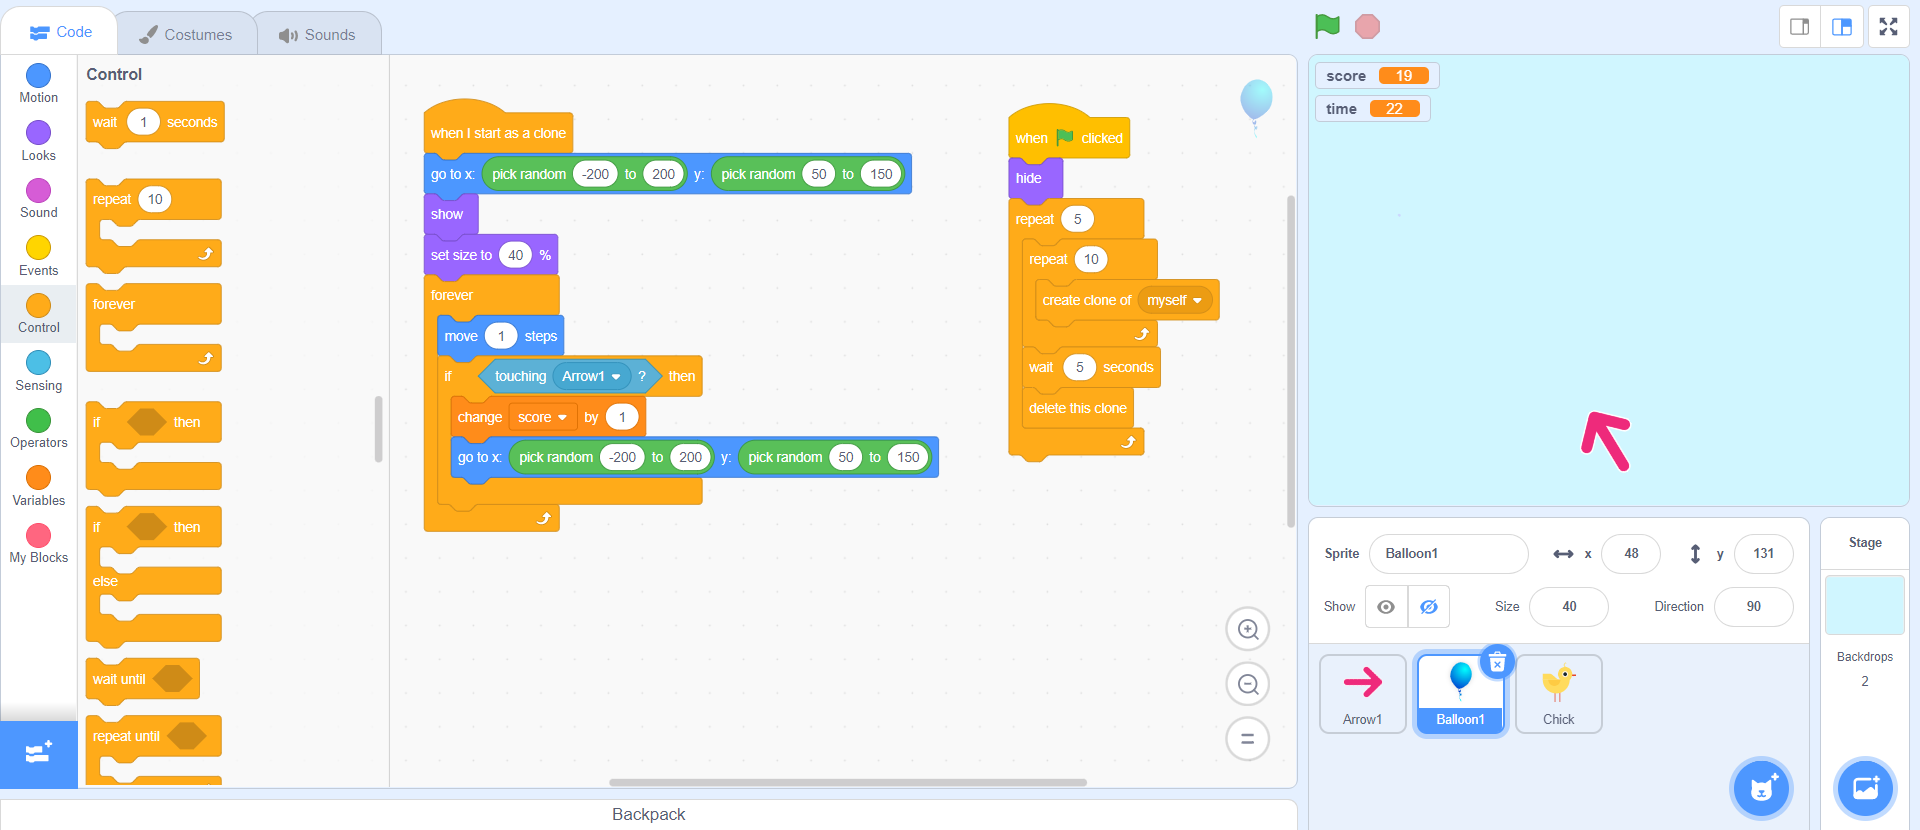
\includegraphics[width=1.0\linewidth,height=0.5\linewidth]{fig090010.png}
   \caption{Increasing score}
\label{fig090010}
\end{figure}

The second check to be made is if the balloon is not hit by the catapult and reaches the end of the screen. It must be checked if the x coordinate is greater than 220. If the condition is true, the clone must be placed on the left side of the screen, and to make the game more attractive, it will also change its costume (color).

\begin{figure}[H]
   \centering
   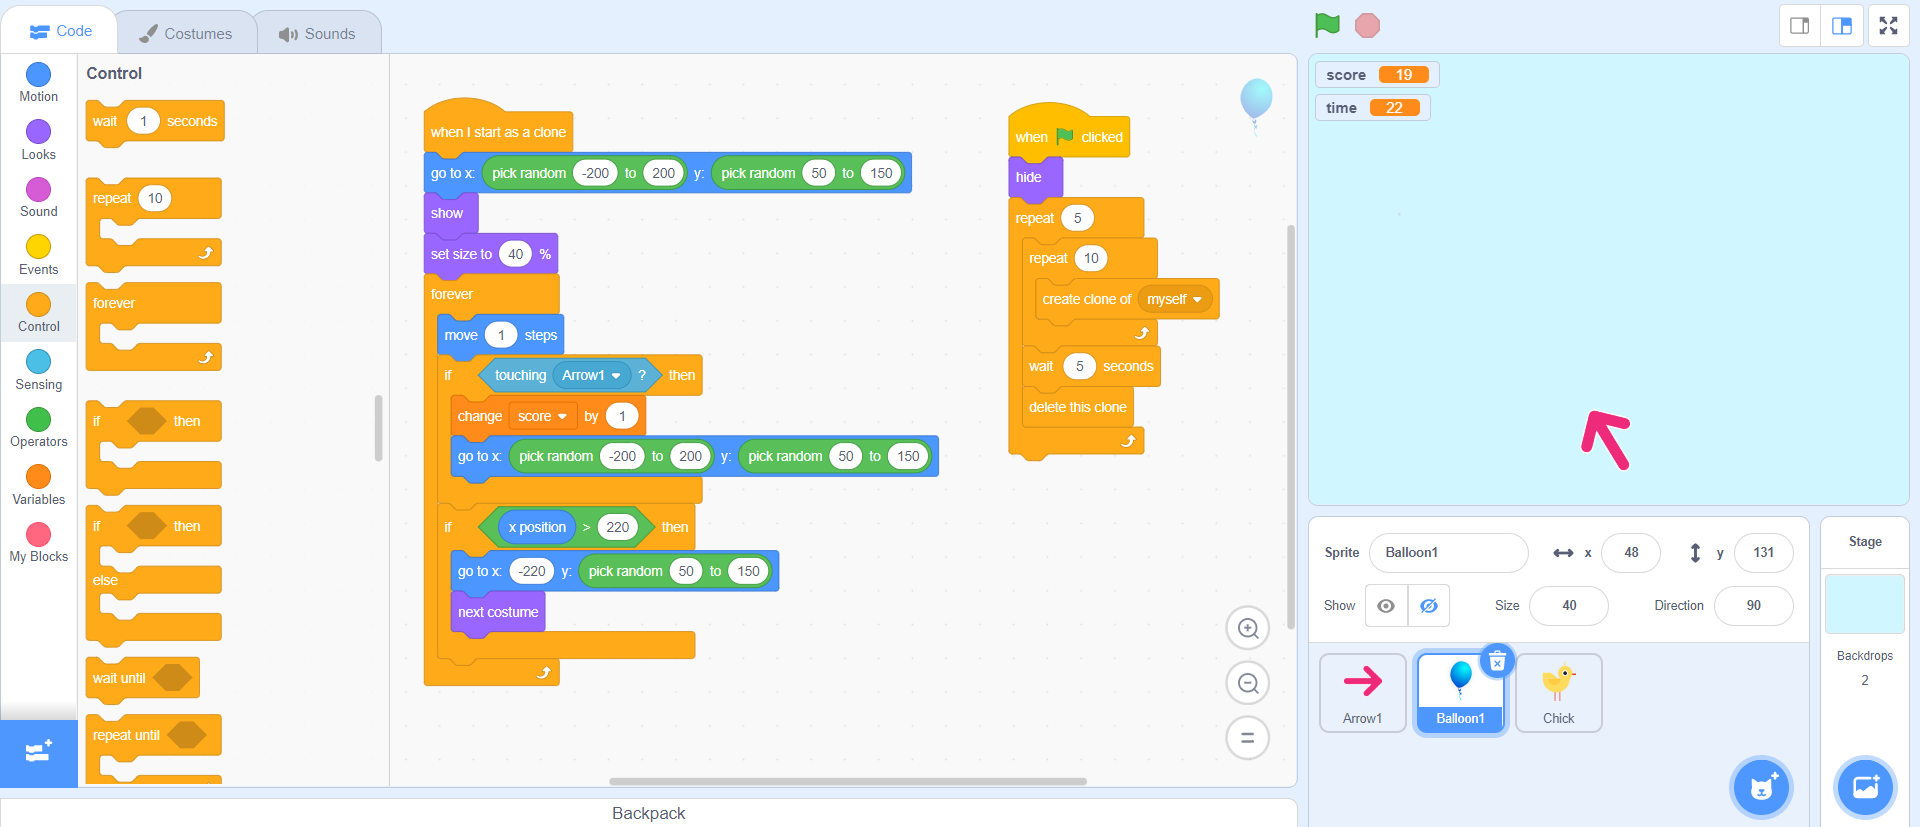
\includegraphics[width=1.0\linewidth,height=0.5\linewidth]{fig090011.png}
   \caption{The Bubble Code}
\label{fig090011}
\end{figure}

The game is almost ready. When launched, clones of the balloon appear and can be burst using the catapult. Also, the time variable decreases, and the result variable increases.

The final step is to program the character to report the final result. When the game starts, this character must be hidden. He should show up when he gets the "stop game" message from the catapult. The instruction to print the result is from the purple group - "thing Hmm... for 2 seconds". The result should be displayed instead of the "Hmm..." message. The "join apple banana" instruction pastes the two words from the green group of instructions. In this game, again, two things need to stick together. One is the message "Your score is," and the second is the value of the score variable.

\begin{figure}[H]
   \centering
   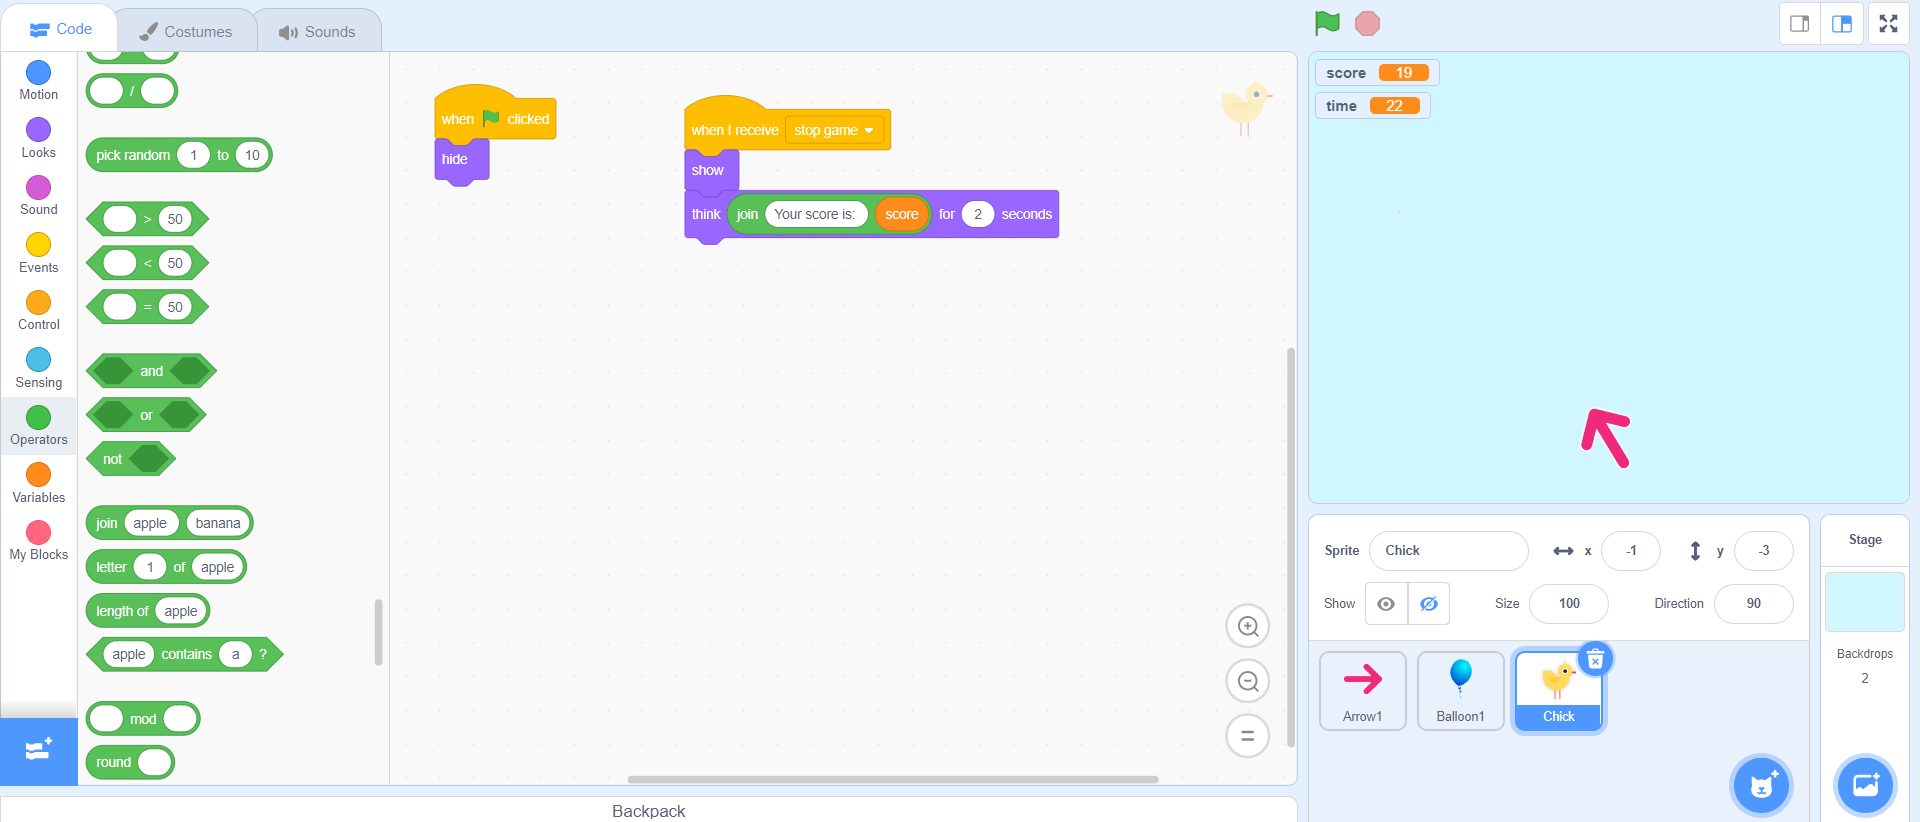
\includegraphics[width=1.0\linewidth,height=0.5\linewidth]{fig090012.png}
   \caption{The character code that announces the result}
\label{fig090012}
\end{figure}

Game over. Play it with your friends to see who can pop the most balloons in 30 seconds.
